Le stage s'intéressant à l'implémentation d'un algorithme d'ordonnacement sur une plateforme hétérogène, une carte possédant un tel processeur est mis à ma disposition. Cette carte se nomme ROCK960 et est fabriquée par l'entreprise \textit{96Boards}. Cette carte de développement contient de nombreuses interfaces mais nous nous contenteront d'utiliser l'interface Série TTL à laquelle nous nous connecterons via un convertisseur USB vers TTL. Cela me permettra d'interfacer via un terminal qui fonctionnera avec une liaison série. 

Au centre de la carte est un \gls{SOC} Rockchip RK3399. Ce processeur contient deux type de cœurs, ou processeurs. Deux d'entre eux sont des processeurs Cortex-A72 et les quatre autres sont des processeurs Cortex-A53. Ces 6 processeurs utilisent le même jeu d'instruction : ARMv8-A 64-bit. Cela sera important par la suite afin de faciliter la migration de tache entre les processeurs, en effet si les jeux d'instructions des processeurs étaient différents, plusieurs copies du code compilé devrait exister tout en maintenant un lien d'équivalence entre les deux codes. Cela est bien au delà de la portée de mon stage mais sera un point intéressant à explorer.

\begin{figure}[H]
    \centering
    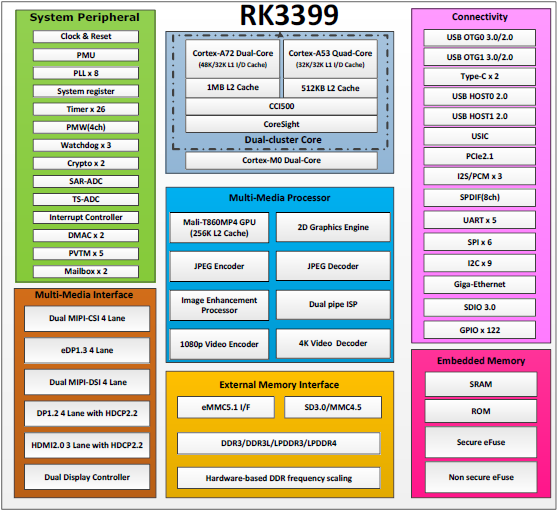
\includegraphics[width=0.45\paperwidth]{Images/RK3399_Block_Diagram.png}
    \caption{Architecture du processeur RK3399}
    \label{fig:archi_rk3399}
\end{figure}

Le SOC RK3399 contient bien d'autres composants et peut interfacer avec de nombreux périphériques (écran HDMI, USB, caméra MPI-CSI, SPI, UART, I2C, etc...) comme le montre la figure \ref{fig:archi_rk3399}. Ce diagramme nous montre aussi que les deux \gls{cluster} de processeurs ne partagent pas les cache L1 ni L2 mais sont interconnectés par une interface CCI-500 qui, selon le site des développeurs ARM, permet la cohérence des caches des deux clusters.